\documentclass[10pt,twocolumn,letterpaper]{article}

\usepackage{cvpr}
\usepackage{times}
\usepackage{epsfig}
\usepackage{graphicx}
\usepackage{amsmath}
\usepackage{amssymb}
\usepackage{listings}

% Include other packages here, before hyperref.

% If you comment hyperref and then uncomment it, you should delete
% egpaper.aux before re-running latex.  (Or just hit 'q' on the first latex
% run, let it finish, and you should be clear).
\usepackage[breaklinks=true,bookmarks=false]{hyperref}

\cvprfinalcopy % *** Uncomment this line for the final submission

\def\cvprPaperID{****} % *** Enter the CVPR Paper ID here
\def\httilde{\mbox{\tt\raisebox{-.5ex}{\symbol{126}}}}

% Pages are numbered in submission mode, and unnumbered in camera-ready
%\ifcvprfinal\pagestyle{empty}\fi
\setcounter{page}{1}
\begin{document}

%%%%%%%%% TITLE
\title{Recent Advances on Traveling Salesman Problem
\thanks{ This work was completed as an artificial intelligence course project at Xi'an Jiaotong University. Permission to copy without all or part of this material is granted provided that the copies are not made or distributed for direct commercial advantage.}
}

\author{Yihui He\\
Xi'an Jiaotong University\\
Xi'an, China\\
{\tt\small heyihui@stu.xjtu.edu.cn}
% For a paper whose authors are all at the same institution,
% omit the following lines up until the closing ``}''.
% Additional authors and addresses can be added with ``\and'',
% just like the second author.
% To save space, use either the email address or home page, not both
\and
Ming Xiang
\thanks{corresponding author.}\\
Xi'an Jiaotong University\\
Xi'an China\\
{\tt\small mxiang@mail.xjtu.edu.cn}
}

\maketitle
%\thispagestyle{empty}

%%%%%%%%% ABSTRACT
\begin{abstract}
With applications to many disciplines, the traveling salesman problem (TSP) is a classical computer science optimization problem with applications to industrial engineering, theoretical computer science, bioinformatics, and several other disciplines. In recent years, there have been a
plethora of novel approaches for approximate solutions ranging from simplistic greedy to cooperative distributed algorithms derived from artificial intelligence. In this paper,
we perform an evaluation and analysis of cornerstone algorithms for the metric TSP. We evaluate the nearest neighbor, greedy, Christofides, and genetic algorithms. We use
several datasets as input for the algorithms including several small datasets, two medium-sized datasets representing
cities in the United States, and a synthetic dataset consisting
of 1,000 cities to test algorithm scalability. We discover that
the nearest neighbor and greedy algorithms efficiently calculate solutions for smaller datasets. Christofides has the best
performance for both optimality and runtime for medium
to large datasets. Genetic algorithms can occasionally find
near-optimal solutions but have no guarantee and generally have longer runtimes.
\end{abstract}

%%%%%%%%% BODY TEXT
\section{Introduction}
Known to be NP-hard, the traveling salesman problem (TSP) was first formulated in 1930 and is one of the most studied optimization problems to date [14]. The problem is as follows: given a list of cities and a distance between each pair of cities, find the shortest possible path that visits every city exactly once and returns to the starting city. The TSP has broad applications including: shortest-path
for lasers to sculpt microprocessors and delivery logistics for mail services, to name a few.

The TSP is an area of active research. In fact, several
variants have been derived from the original TSP. In this
paper, we focus on the metric TSP. In the metric TSP, all
distances between cities satisfy the triangle inequality. That
is, for three cities, A, B, and C:
\begin{equation}
	dist(A, C) < dist(A, B) + dist(B, C)
\end{equation}
This simplification allows us to survey several cornerstone algorithms without introducing complex scenarios, specifically
for Christofides. The remainder of this paper is organized
as follows. In Section 2, we briefly review the first solutions
and survey modern approaches and variants to the TSP. We
describe the algorithms used in our experiment and outline
key implementation details in Section 3. A description of
the benchmark datasets and results of the experiment are
detailed in Section 4. A discussion in Section 5 explains the
findings and compares the performance of the algorithms.
We then conclude and describe future work in Section 6.

\section{Background}
An example TSP is illustrated in Figure \ref{fig:egtsp}. The input is
shown in subfigure (a) as a collection of cities in the twodimensional space. This input can be represented as a distance matrix for each pair of cities or as a list of points
denoting the coordinate of each city. In the latter method,
distances are calculated using Euclidean geometry. A nonoptimal tour is shown in subfigure (b). Although not shown
in the figure, each edge will have some non-negative edge
weight denoting the distance between two nodes or cities.
Due to the computational complexity of the TSP, it may be
necessary to approximate the optimal solution. The optimal
tour is shown in subfigure (c). For small graphs, it may be
possible to perform an exhaustive search to obtain the optimal solution. However, as the number of cities increases, so
does the solutions space, problem complexity, and running
time.

\begin{figure}
\centering
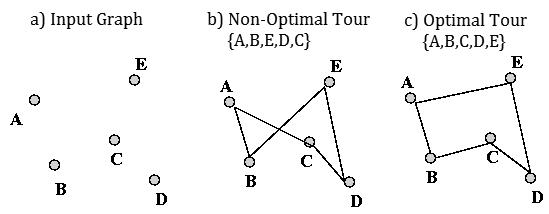
\includegraphics[width=0.7\linewidth]{egtsp}
\caption{}
\label{fig:egtsp}
\end{figure}

Figure 2 lists the number of edges and total possible num-
ber of tours for a specific dataset size. The number of possi-
ble tours is (n − 1)!/2 since the same tour, with start point
X and Y appears twice: once with X as the start node and
once with Y as the start node.

Mathematical problems similar to the Traveling salesman
problem date back to the 18th century. The basis of the
problem was first discussed by Irish mathematician William
Rowan Hamilton and by a British mathematician Thomas
Penyngton Kirkman.

The TSP problem itself was first formulated in the 1930s
by Karl Menger in Vienna and Harvard. It was later studied
by statisticians Mahalanobis, Jessen, Gosh, and Marks for
agricultural applications. The problem was then popular-
ized by mathematician Merill Flood with his colleagues at
Research and Development Corporation in the 1940s. By
the mid-1950s, solutions for TSP began to appear. The first
solution was published by Dantzig, Fulkerson, and Johnson
using a dataset of 49 cities. The progression of solutions is
shown in Figure 3. In 1972, Richard M. Karp proved that
the Hamiltonian cycle problem was NP-Complete, which
proves that the TSP is NP-Hard.

In modern day, the traveling salesman problem has a va-
riety of applications to numerous fields. Examples among
these applications include genome sequencing, air traffic con-
trol, supplying manufacturing lines, and optimization.

\subsection{TSP Variants}
Several variants of the original TSP exist. Some of these
variants differ in their representation of cities and some differ
by the constraints placed on city distances. We describe the
Euclidean, Graphic, and Asymmetric TSP variants in this
section.
\subsubsection{Euclidean TSP}
In the Euclidean TSP, the input is given as a list of coor-
dinates describing the location of each city in R 2 [1]. It is
possible to extend this into higher dimensions as well. The
alternative to giving a list of city coordinates is to give a
distance/adjacency matrix describing the distances between
each city pair. It is possible to derive the distance ma-
trix given the city coordinates using Euclidean geometry.
However, given the distance matrix, inferring the coordi-
nates is not as straightforward and requires computation of
a Gramian matrix and application of several matrix decom-
position methods
\
\subsubsection{Graphic TSP}
In recent years, the graphic TSP has attracted attention
from the research community. The graphic TSP problem
asks for the shortest tour that visits each vertex at least
once. The current best approximation algorithm returns a
solution within 13/9 ≈ 1.444 of the optimal [16]. For the
past 30 years, Christofides had been the leading algorithm
with a 1.5 approximation. Although the 13/9 approximation
is for a TSP variant, it is an important milestone for TSP
approximations nonetheless.

\subsubsection{Asymmetric TSP}
All TSP variants described thus far have assumed an undi-
rected graph, resulting in cost(A, B) = cost(B, A). The
asymmetric TSP introduces directed edges. As a conse-
quence, algorithms with assumptions about reflexive dis-
tances may fail when cost(A, B) 6 = cost(B, A). Real world
applications of this includes roads and highways – specif-
ically the case of one-way streets, detours, and alternate
routes. Additionally when modeling vehicle energy usage,
the geographical topology makes traveling uphill cheaper
than downhill despite traveling between the same two points.

\subsection{Related Heuristics}
In this section, we briefly summarize current approaches
for the metric TSP. We describe the 2-approximation algo-
rithm and survey an advanced technique based on artificial
intelligence.
\subsubsection{2-Approximation Algorithm}
A simple two-approximation solution can be achieved by
constructing a minimum spanning tree (MST) for the input
TSP graph and creating a list of vertices (no duplicates)
from a pre-order walk of the MST [20]. This list of vertices
becomes a Hamiltonian cycle and is a solution to the TSP.
This algorithm completes in polynomial time and is is guar-
anteed to return a two-approximation solution (see [20] for
proof).

\subsubsection{Ant-Colony Approach}
Classified under the umbrella of nature-inspired algorithms,
the ant colony system (ACS) is a distributed swarm intelli-
gence algorithm that has a set of cooperating agents called
ants that attempt to solve the TSP. This method attempts
to mimic how ants find the shortest path from their home to
food in real life. In ACS, ants communicate by depositing
pheromones on the graph edges as they build TSP solu-
tions [7]. Over time, the shorter paths build larger amounts
of pheromones. The solution to the TSP is the path with
highest pheromone levels which visit every city.

This algorithm is able to run on both symmetric and
asymmetric TSPs. For the symmetric TSP with 170 cities
or less, the ACS algorithm finds the optimum solution. For
the asymmetric TSP with 170 cities or less, it found a so-
lution within 0.40% of the optimal and outperforms genetic
algorithm approaches [7].
%-------------------------------------------------------------------------
\section{Algorithms}
e now move to a discussion of the algorithms used in
our evaluation. First, we describe the traditional nearest
neighbor and greedy approaches in Sections 3.1 and 3.2. We
then outline Christofides algorithm in Section 3.3 and then
discuss the genetic algorithm in Section 3.4.

\subsection{Random Path}
Finding the worst case of TSP is as hard as the best one.
So we randomly generate a random path, 
and use this as a lower bound benchmark for all other algorithms.

\subsection{Greedy Algorithm}
The greedy heuristic is based on Kruskal’s algorithm to
give an approximate solution to the TSP [13]. The algorithm
forms a tour of the shortest route and can be constructed if
and only if:
The edges of the tour must not form a cycle unless
the selected number of edges is equal to the number of
vertices in the graph.
The selected edge (before being appended to the tour)
does not increase the degree of any node to be more
than 2.
The algorithm begins by sorting all edges from least weight
to most heavily weighted. After the edges are sorted, the
least heavily-weighted edge is selected and it is added to the
tour if it does not violate the above conditions. The algo-
rithm continues by selecting the next least-cost edge and
adding it to the tour. This process is repeated until all ver-
tices can be reached by the tour. The result is a minimum
spanning tree and is a solution for the TSP. The runtime for
the greedy algorithm is O(n 2 log(n)) and generally returns a
solution within 15-20\% of the Held-Karp lower bound [17].

\subsection{2opt Algorithm}
In optimization, 2-opt is a simple local search algorithm first proposed
by Croes in 1958 for solving the traveling salesman problem\cite{croes1958method}.
The main idea behind it is to take a route that crosses over itself and reorder it so that it does not.
A complete 2-opt local search will compare every possible valid combination of the swapping mechanism. This technique can be applied to the travelling salesman problem as well as many related problems. These include the vehicle routing problem (VRP) as well as the capacitated VRP, which require minor modification of the algorithm.

2-Opt, First create a random tour, and then optimize this with the 2-opt
algorithm. 
In a 2opt optimization step we consider two nodes, Y and X.  (Between Y
and X there might be many more nodes, but they don't matter.) We also
consider the node C following Y and the node Z following X. i
For the optimization we see replacing the edges CY and XZ with the edges CX
and YZ reduces the length of the path  C -> Z.  For this we only need to
look at |CY|, |XZ|, |CX| and |YZ|.   |YX| is the same in both
configurations.

If there is a length reduction we swap the edges AND reverse the direction
of the edges between Y and X.
 
In the following function we compute the amount of reduction in length
(gain) for all combinations of nodes (X,Y) and do the swap for the
combination that gave the best gain.
 
This pseudocode is shown below.

\begin{lstlisting}
repeat until no improvement is made {
start_again:
best_distance = calculateTotalDistance(existing_route)
for (i = 0; i < number of nodes eligible to be swapped - 1; i++) {
   for (k = i + 1; k < number of nodes eligible to be swapped; k++) {
       new_route = 2optSwap(existing_route, i, k)
       new_distance = calculateTotalDistance(new_route)
       if (new_distance < best_distance) {
	   existing_route = new_route
	   goto start_again
       }
   }
}
}
\end{lstlisting}

\subsection{Genetic Algorithm}
Genetic algorithms (GA) are search heuristics that at-
tempt to mimic natural selection for many problems in op-
timization and artificial intelligence [4]. In a genetic algo-
rithm, a population of candidate solutions is evolved over
time towards better solutions. These evolutions generally
occur through mutations, randomization, and recombina-
tion. We define a fitness function to differentiate between
better and worse solutions. Solutions, or individuals, with
higher fitness scores are more likely to survive over time.
The final solution is found if the population converges to a
solution within some threshold. However, great care must
be taken to avoid being trapped at local optima.

We will now apply a genetic algorithm to the traveling
salesman problem [2]. We define a fitness function F as the
length of the tour. Supposed we have an ordering of the
cities A = {x 1 , x 2 , ..., x n } where n is the number of cities.
The fitness score for the TSP becomes the cost of the tour
d(x, y) denote the distance from x to y.
\begin{equation}
	F(A) =\sum_{i=0}^{n-1} d(x_i , x_{i+1}) + d(x_n , x_0 )
\end{equation}
The genetic algorithm begins with an initial, P 0 , random
population of candidate solutions. That is, we have a set of
paths that may or may not be good solutions. We then move
forward one time step. During this time step, we perform a
set of probabilistic and statistical methods to select, mutate,
and produce an offspring population, P 1 , with traits similar
to those of the best individuals (with the highest fitness)
from P 0 . We then repeat this process until our population
becomes homogeneous.

The running time of genetic algorithms is variable and de-
pendent on the problem and heuristics used. However, for
each individual in the population, we require O(n) space for
storage of the path. For genetic crossover, the space require-
ment remains O(n). The best genetic algorithms can find
solutions within 2% of the optimal tour for certain graphs
[10].

\section{Implementation}
\subsection{Greedy Algorithm}
The greedy solution to TSP differs from the nearest neigh-
bor heuristic because it uses a Kruskal’s approach to the
problem. Instead of starting at a random node and building
a tour using the nearest neighbor of the selected node, the
Greedy algorithm selects the least weighted edge and adds
it to the tour regardless of if it is connected or disconnected
to the current tour.

The Greedy algorithm was implemented in Java and is
available on Github 1 . The program reads the input datasets
from the files and constructs a distance matrix correspond-
ing to distances between cities. The algorithm first sorts
all of the weights of the edges from lowest to most heav-
ily weighted, and selects the lightest edge to begin the tour
with. It then selects the next lightest edge and adds it to
the tour as long as it doesn’t create a cycle or make any
vertices have a degree of more than 2. The algorithm keeps
performing the loop until the number of edges in the tour is
equal to the number of vertices in the graph. It then prints
out all of the edges added to the tour, the running time of
the operation, and returns the path cost of the tour.

\section{Experiment}
We benchmark our algorithms using publicly available
datasets. 
Additionally, to test the scalability of the algorithms, we generated a synthetic dataset consisting of 200 cities. 
In all dataset names, the numeric digits represent
the number of cities in the dataset. 
The datasets are as follows: P15, ATT48, and R200.
All datasets except R200 can be found online \cite{data0}\cite{data1}. The
ATT48 and SGB128 datasets represent real-data consisting
of locations of cities in the United States. 
A visual representation of the ATT48 dataset in the 2D plane is shown
in Figure \ref{fig:00001}
\begin{figure}
\centering
\includegraphics[width=\linewidth]{../TSP_Animation/00001.png}
\caption{the ATT48 dataset in the 2D plane. (the United States)}
\label{fig:00001}
\end{figure}

Not all datasets have a known optimal tour. When this is the case, we use random path algorithm to infer a upper bound of the optimal tour. 

\subsection{Random Dataset}
The R200 dataset was generated by plotting 200 random, 
uniformly distributed points (x, y), in $R^2$ with $(x, y) \in
[0, 1000]$. As a result, all
distances satisfy the triangle inequality and this dataset can
be classified as a metric TSP dataset. The running time
for creating the dataset is $O(n)$. 
The output is a list of all cities represented as $(x,y)$ points.

\subsection{Comparison}
As we can see in Figure 7a, the nearest neighbor and
greedy algorithms have similar solution costs. In Figure 7b,
we can see that most algorithms return a solution under 20%
over the optimal for small datasets and are often twice the
optimal for larger datasets.
\begin{figure}
\centering
\includegraphics[width=\linewidth]{../TSP_Animation/time.pdf}
\caption{runtime comparison, the y axis is in log scale}
\label{fig:tsp}
\end{figure}

In terms of running time (Figure \ref{fig:length}), the best algorithm
is nearest neighbor. However, in terms of optimal cost of
solution, the best algorithm is greedy. This is in line with our
expectations and alludes to the fact that different heuristics
are better suited for different situations
\begin{figure}
	\centering
	\includegraphics[width=\linewidth]{../TSP_Animation/length.pdf}
	\caption{tour length comparison, the y axis is in log scale, divided by random tour length}
	\label{fig:length}
\end{figure}
We found that the nearest neighbor calculated a route
for even the largest dataset (1000 cities) in 4 seconds, prov-
ing that this algorithm can quickly calculate a solution for
larger traveling salesman problems. However, at that scale,
the route for the solution was almost double the cost of
the optimal solution. Thus, the nearest neighbor is a poor
heuristic choice for extremely large datasets. Furthermore,
this heuristic is best suited for smaller routes when any op-
timization gains are marginal in comparison to time com-
plexity of other, more sophisticated heuristics.

As shown in Figure 7a, Christofides algorithm performs
fairly consistently, in comparison to the nearest neighbor
and greedy algorithms, across all datasets. Highlighted in
Figure 8, the running time of Christofides is generally a fast
algorithm for small to medium datasets and is the fastest al-
gorithm for the G1000 dataset. This suggests that for larger
datasets, if running time is a concern, then the Christofides
algorithm should be used. Figure 7b further demonstrates
that Christofides algorithm maintains a smaller percent above
optimal than the other algorithms. From this, we can see
that Christofides algorithm has high accuracy and faster
runtimes than other heuristics, especially for larger datasets.

Since the genetic algorithm does not have an optimality
guarantee, its results vary across datasets. It can perform
very well – as demonstrated on the FRI26 dataset where it
returned a solution with 3.31% of the optimal. On the other
hand, it returned the worst solution for three out of the seven
datasets. For both the GR17 and WG59 datasets, the ge-
netic algorithm returned a solution of an order of magnitude
greater than the optimal. Due to the randomized nature of
genetic algorithms, it may be possible to become stuck at a
local optimum. This may have been the case for the G1000
dataset. The other three algorithms were within 2× the
optimal.

From a running time standpoint, the genetic algorithm
takes the longest time to reach a solution. For most datasets,
the algorithm required ten seconds to one minute to com-
plete. This can be attributed to the forward progress ep-
silon, that is the threshold at which we declare a population
as “no longer evolving.” The smaller the epsilon, the longer
the runtime. Although genetic algorithms have longer run-
times, it may be possible to find a solution better than the
other three algorithms.

\section{Conclusion}
Most of our algorithms attempt to solve the TSP in a
linear fashion. Originating from artificial intelligence, the
genetic algorithm is very different compared to greedy, near-
est neighbor, and Christofides. Literature suggests that the
best algorithms focus on iteration and convergence to find
optimal tours – something genetic algorithms attempt to
achieve. For example, the Large Step Markov Chain [11]
relies on Markov chains to find convergence of many paths
to form a global optimum and several papers cite Markov
Chains as the best known solution to TSP. Recent studies in-
clude using adaptive Markov Chain Monte Carlo algorithms
[18]. Many of these extend the Metropolis algorithm [9], a
simulated annealing algorithm which attempts to mimic ran-
domness with particles as the temperature varies. This fur-
ther supports our conclusion that algorithms inspired from
artificial intelligence perform well for finding solutions for
the TSP. However, these may not be suitable when a guar-
antee is required.

As future work, we believe it would be an interesting exer-
cise to add an iterative component to our basic algorithms.
For example, in nearest neighbor, it would be interesting for
the algorithm to evaluate its path efficiency in real time and
backtrack if the path exceeds a certain threshold of costs –
similar to graph search algorithms. Of course, for this kind
of iteration, it would be required to know the optimal cost.
Our work relied on the Christofides algorithm to assume a
lower bound and a similar algorithm could be used to infer
an optimal solution.

In this paper, we surveyed several key cornerstone ap-
proaches to the traveling salesman problem. We selected
four well-known algorithms and tested their performance on
a variety of datasets. Our results suggest that genetic al-
gorithms (and other approaches from artificial intelligence)
are able to find a near-optimal solution. However, these ap-
proaches do not provide guarantees like Christofides and the
two approximation algorithms.

{\small
\bibliographystyle{ieee}
\bibliography{egbib}
}

\end{document}
